\section{Dataset Analysis}
\label{sec:dataset_analysis}

We introduce the MultiEMiT corpus, a multi-layered multimodal dataset of Italian Twitter commentary gathered during live television broadcasts. The data originates from the M.EMO.RAI project \cite{memorai}, which set out to track audience emotional responses in real time. Rather than restricting annotations to positive or negative sentiment, MultiEMiT applies an expanded eight-emotion taxonomy derived from Plutchik's psychoevolutionary model \cite{Plutchik}.

MultiEMiT draws from two television broadcasts representing contrasting formats and registers:

\textit{ProSAT:} Twitter commentary on \textit{Propaganda Live}, a satirical talk show on LA7 combining investigative journalism and political commentary \cite{propagandalive}. The collection captures the broadcast of November 19, 2021, when host Diego Bianchi reported live from the Poland--Belarus border during a humanitarian crisis. The gravity of the event prompted solemn reactions dominated by indignation, grief, and civic debate.

\textit{EMiT (Pechino Express):} Collected as an extension of the EVALITA EMiT benchmark \cite{emit}, this sub-corpus covers \textit{Pechino Express}, an adventure reality show broadcast on Rai2 \cite{pechinoexpress}. Collected during the season premiere on February 11, 2020, viewer discourse centers on lighthearted entertainment, contestant rivalries, and humorous commentary.

Both partitions share an identical structure: a purely textual partition and a multimodal partition pairing the text with its attached media (screenshots, edited images, and memes). This paired structure allows direct comparison between unimodal and multimodal models, showing where visual content modulates the written post. In addition to MultiEMiT, we use the external textual EMiT corpus (5,966 posts across multiple programs \cite{emit}) as supplementary training data for baseline emotion encoders.

Annotation was conducted on Sensitag, a web annotation platform developed at the University of Turin. Each post was evaluated independently by three annotators with backgrounds in computer science or linguistics. Final labels were assigned by majority vote (at least two out of three annotators agreeing).

The corpus is annotated across five pragmatic dimensions:
\begin{itemize}
    \item \textbf{Emotions:} Ten affective categories based on Plutchik's model \cite{Plutchik} (\textit{Joy}--\textit{Sadness}, \textit{Trust}--\textit{Disgust}, \textit{Fear}--\textit{Anger}, \textit{Surprise}--\textit{Anticipation}), supplemented with \textit{Love} and \textit{Neutral}. This task is multi-label, allowing posts to carry multiple concurrent emotional states.
    \item \textbf{Irony and Sarcasm:} Three exclusive classes separating literal statements (\textit{Unironic}), humorous figurative inversion (\textit{Irony}), and hostile, denigratory mockery (\textit{Sarcasm}).
    \item \textbf{Hate Speech:} Identifies abusive language, insults, or harassment directed at individuals or protected groups.
    \item \textbf{Target:} Distinguishes whether comments address the broadcast \textit{Content} (political issues, guests, or news events) or the \textit{Container} (the studio host, network, or production execution).
    \item \textbf{Semiotic Relation:} Categorizes multimodal document intent \cite{MultiM} into \textit{Additive} (modality enrichment), \textit{Parallel} (redundant information), and \textit{Divergent} (ironic contrast or meme dissonance).
\end{itemize}

Sarcasm and emotion in short social media posts are inherently ambiguous. Read in isolation, a comment on the border crisis such as \textit{``Terrible, I am ashamed to be European''} could be seen as shame (\textit{Disgust} + \textit{Fear}), contempt (\textit{Anger} + \textit{Disgust}), or disapproval (\textit{Surprise} + \textit{Sadness}).

Providing annotators with the attached image resolved much of this ambiguity, substantially lifting inter-annotator agreement (Fleiss' $\kappa$) across most emotion labels. Seeing photos of shivering refugees grounded the context, directing consensus toward sadness and distress. This empirical finding provides direct justification for multimodal modeling: if visual context clarifies ambiguous intent for human annotators, multimodal neural architectures should benefit from the same disambiguating cues.

Following gold-standard consolidation, the MultiEMiT corpus resulted in two main partitions: a purely \textbf{Textual} dataset comprising 2,909 posts, and a \textbf{Multimodal} dataset comprising 645 posts with paired image attachments. 

As typical of social media discourse, label distributions exhibit pronounced class imbalance. Tables~\ref{table:text_dist} and~\ref{table:multi_dist} present the complete distribution of labels across both partitions, broken down by broadcast sub-corpus.

\begin{table}[!t]
\centering
\caption{Label Distribution in the MultiEMiT Textual Dataset (2,909 Posts)}
\label{table:text_dist}
\begin{tabular}{l c c c}
\hline
\textbf{Label} & \textbf{Total (2,909)} & \textbf{ProSAT} & \textbf{EMiT} \\
\hline
\multicolumn{4}{l}{\textit{Emotions (multi-label)}} \\
\hline
Love & 340 & 119 & 221 \\
Anticipation & 201 & 75 & 126 \\
Disgust & 410 & 207 & 203 \\
Trust & 613 & 281 & 332 \\
Joy & 552 & 257 & 295 \\
Neutral & 321 & 31 & 290 \\
Fear & 55 & 44 & 11 \\
Anger & 163 & 121 & 42 \\
Surprise & 486 & 225 & 261 \\
Sadness & 255 & 211 & 44 \\
\hline
\multicolumn{4}{l}{\textit{Irony}} \\
\hline
Irony & 481 & 237 & 244 \\
Unironic & 2,072 & 828 & 1,244 \\
Sarcasm & 41 & 15 & 26 \\
\hline
\multicolumn{4}{l}{\textit{Offensiveness}} \\
\hline
Offensive & 52 & 31 & 21 \\
\hline
\multicolumn{4}{l}{\textit{Target}} \\
\hline
Container & 1,147 & 343 & 804 \\
Content & 1,138 & 710 & 428 \\
\hline
\end{tabular}
\end{table}

\begin{table}[!t]
\centering
\caption{Label Distribution in the MultiEMiT Multimodal Dataset (645 Posts)}
\label{table:multi_dist}
\begin{tabular}{l c c c}
\hline
\textbf{Label} & \textbf{Total (645)} & \textbf{ProSAT} & \textbf{EMiT} \\
\hline
\multicolumn{4}{l}{\textit{Emotions (multi-label)}} \\
\hline
Love & 50 & 17 & 33 \\
Anticipation & 61 & 10 & 51 \\
Disgust & 78 & 18 & 60 \\
Trust & 214 & 82 & 132 \\
Joy & 168 & 79 & 89 \\
Neutral & 90 & 21 & 69 \\
Fear & 4 & 4 & 0 \\
Anger & 34 & 29 & 5 \\
Surprise & 82 & 24 & 58 \\
Sadness & 25 & 23 & 2 \\
\hline
\multicolumn{4}{l}{\textit{Irony}} \\
\hline
Irony & 109 & 21 & 88 \\
Unironic & 516 & 199 & 317 \\
Sarcasm & 20 & 5 & 15 \\
\hline
\multicolumn{4}{l}{\textit{Offensiveness}} \\
\hline
Offensive & 6 & 3 & 3 \\
\hline
\multicolumn{4}{l}{\textit{Target}} \\
\hline
Container & 395 & 103 & 292 \\
Content & 199 & 85 & 114 \\
\hline
\multicolumn{4}{l}{\textit{Semiotic Relation}} \\
\hline
Additive & 389 & 158 & 231 \\
Divergent & 158 & 42 & 116 \\
Parallel & 100 & 10 & 90 \\
\hline
\end{tabular}
\end{table}

Across both partitions, the most frequent affective states are \textit{Trust} and \textit{Joy}, indicating an overall positive engagement with broadcast programming. However, negative emotions exhibit marked domain dependency: \textit{Sadness}, \textit{Anger}, and \textit{Fear} are heavily concentrated within ProSAT due to the geopolitical reportage, whereas they remain negligible in the lighthearted Pechino Express subset.

Similarly, irony displays genre-specific dynamics. In the multimodal corpus, irony is prevalent in Pechino Express (88 instances) despite Propaganda Live being a satirical format. This occurs because the specific Propaganda Live episode under study addressed an acute humanitarian crisis, prompting solemn reflection rather than playful sarcasm. Regarding semiotic relations, the \textit{Additive} relation dominates in both subsets, while \textit{Parallel} and \textit{Divergent} relations appear far more frequently in entertainment contexts where visual memes thrive.

\begin{figure*}[!t]
\centering
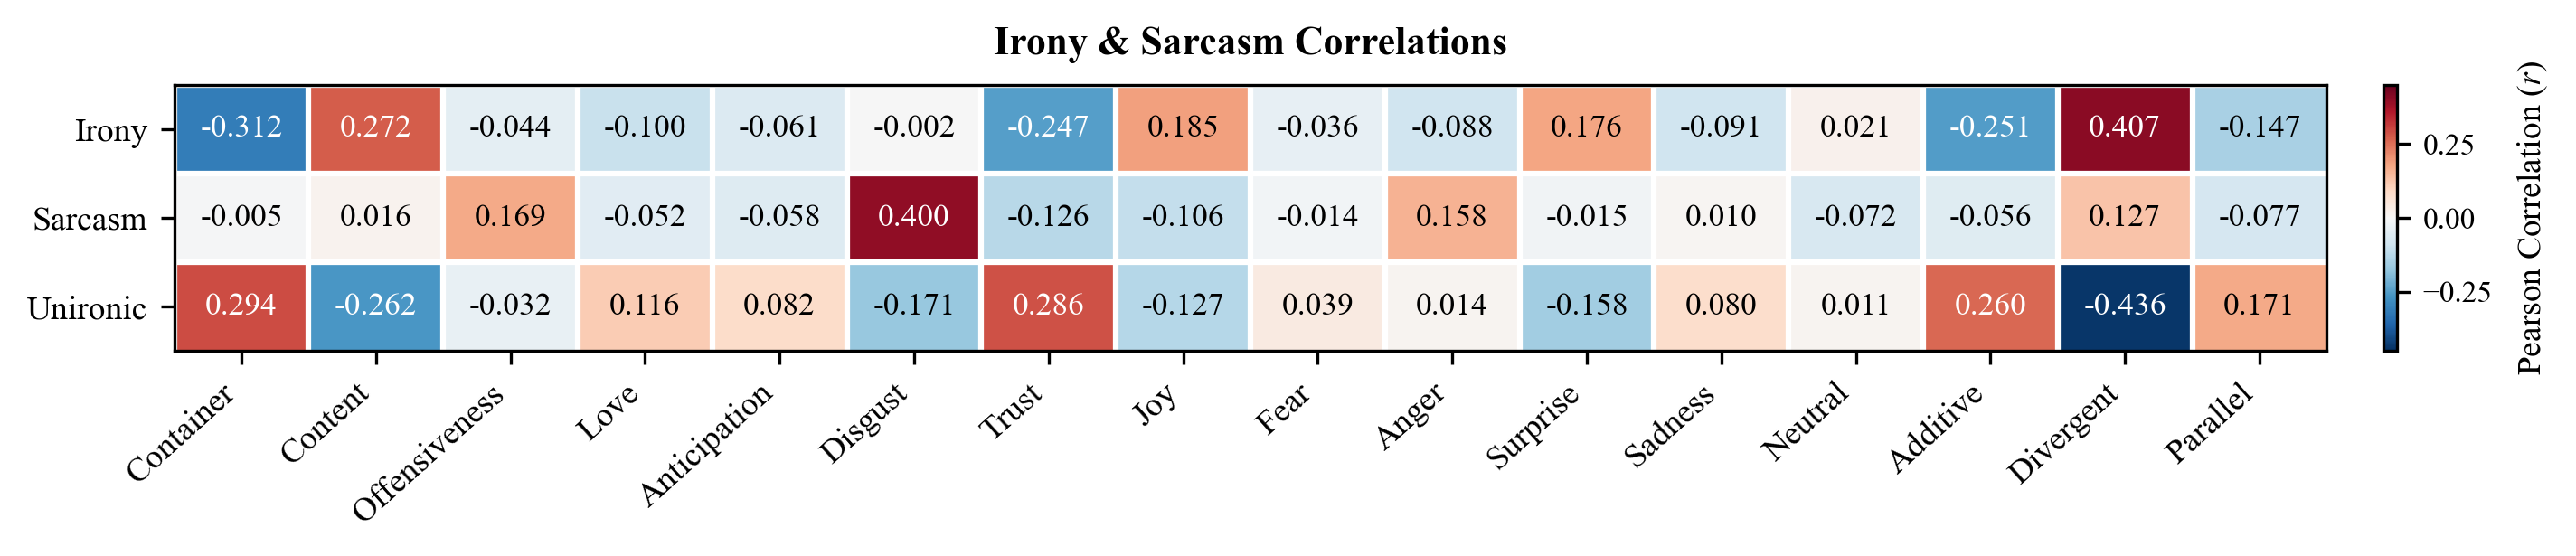
\includegraphics[width=\textwidth]{imgs/irony_correlations_english.png}
\caption{Pearson correlation matrix for the irony and sarcasm dimension across multi-level annotations.}
\label{fig:irony_correlations}
\end{figure*}

\begin{figure*}[!t]
\centering
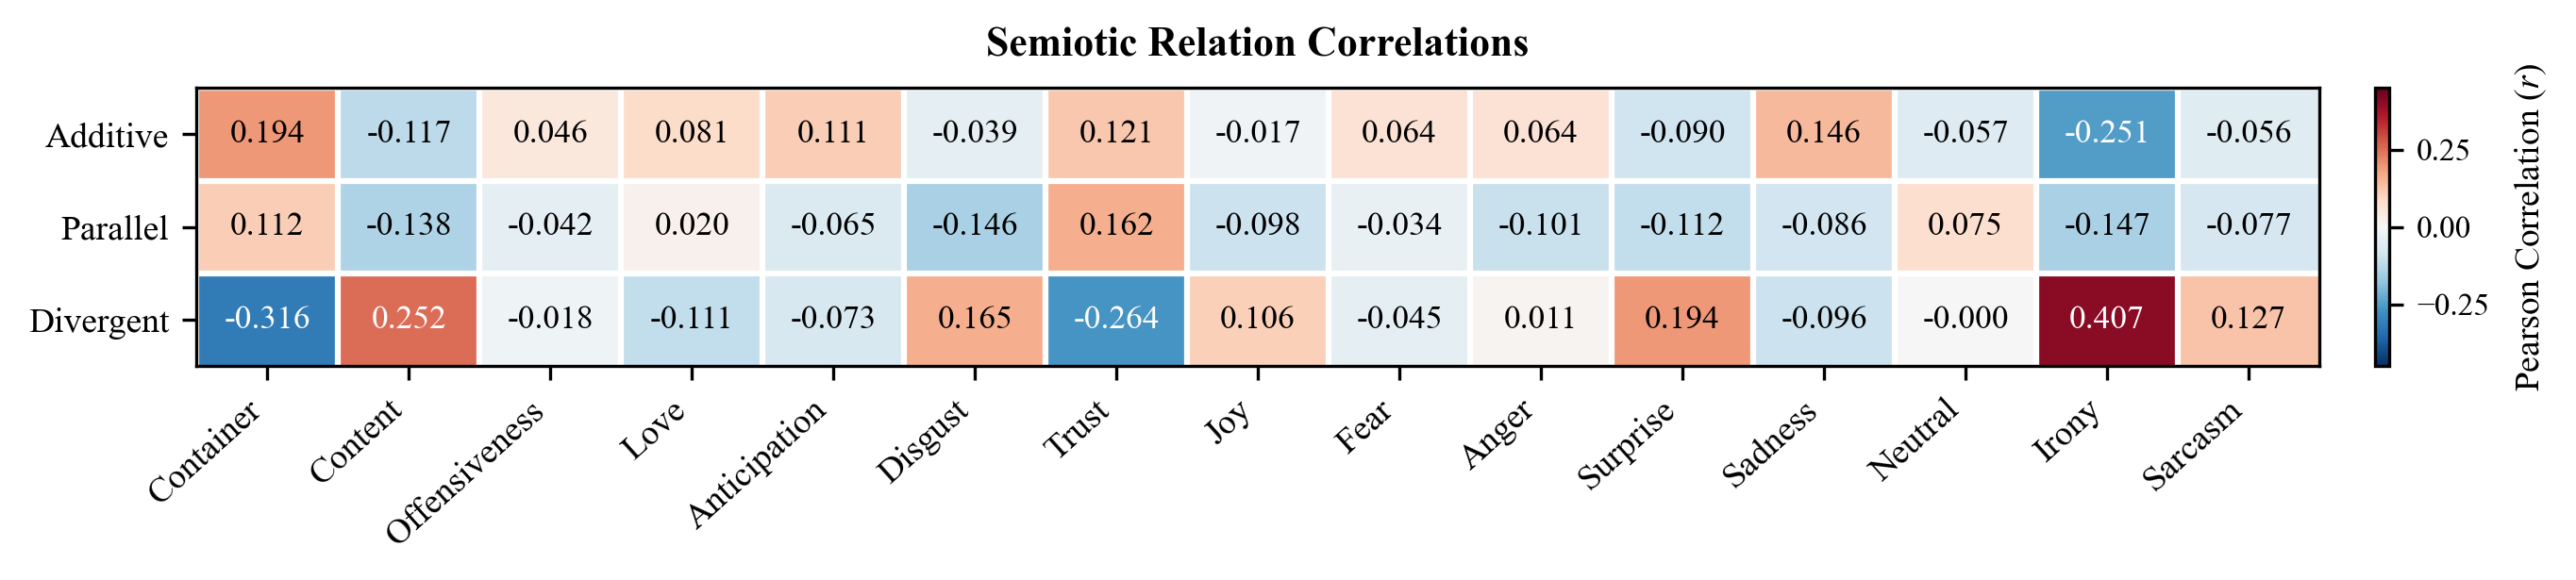
\includegraphics[width=\textwidth]{imgs/relation_correlations_english.png}
\caption{Pearson correlation matrix for semiotic text--image relations against contextual and affective markers.}
\label{fig:relations_correlations}
\end{figure*}

The multi-layered annotation of MultiEMiT enables systematic investigation into the statistical dependencies connecting emotional, figurative, and semiotic dimensions. By computing Pearson correlation coefficients ($r$) across all label pairs, we identified pronounced interdependencies indicating that pragmatic categories act as strong mutual predictors.

\begin{figure}[!t]
\centering
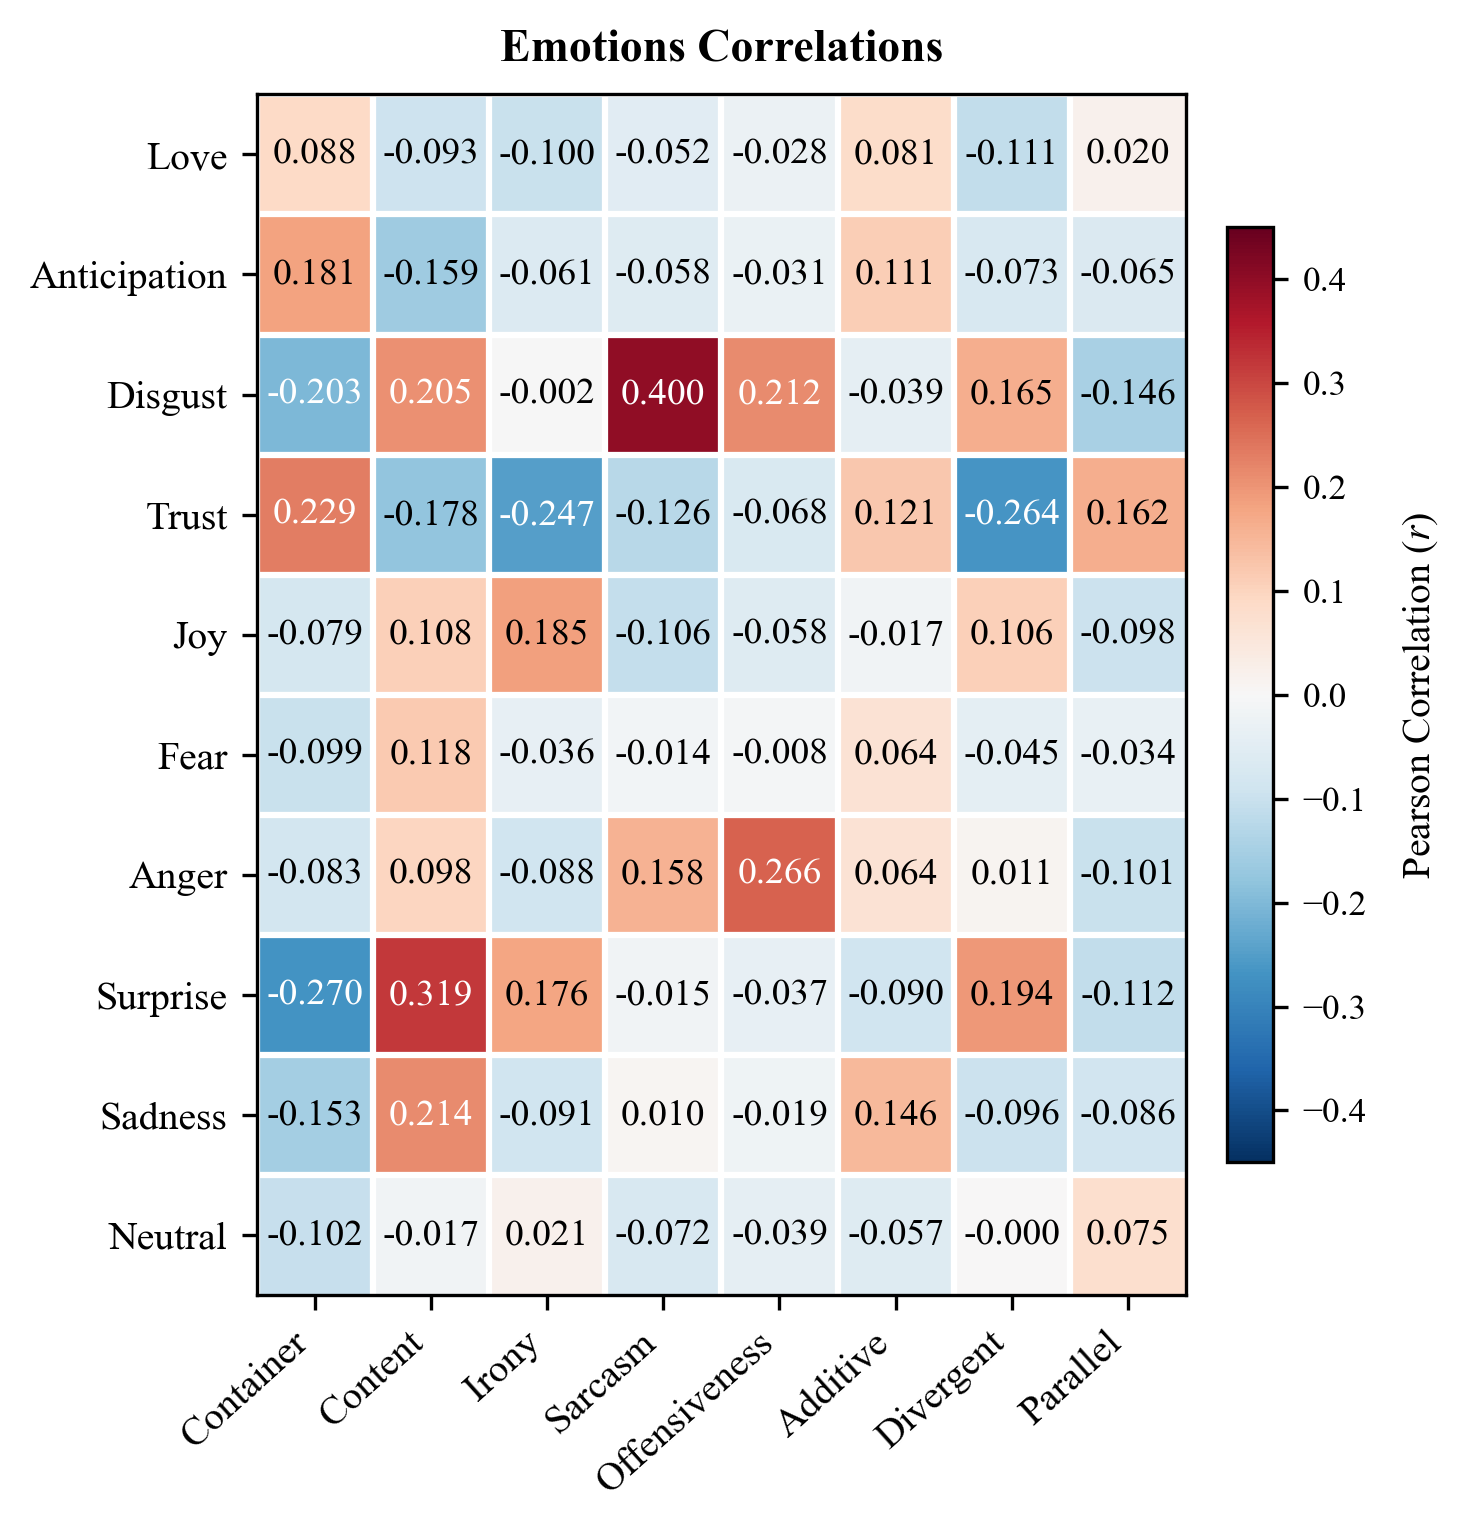
\includegraphics[width=0.92\columnwidth]{imgs/emotion_correlations_english.png}
\caption{Emotions Correlations: Pearson correlation matrix between emotion labels and contextual dimensions (broadcast targets, figurative speech, and semiotic relations).}
\label{fig:emotions_correlations}
\end{figure}

Examining the correlation matrix for \textbf{Emotions} (Fig.~\ref{fig:emotions_correlations}), a clear dichotomy emerges between the \textit{Container} and \textit{Content} targets. Program-directed affective states (\textit{Trust} $r = 0.229$, \textit{Anticipation} $r = 0.181$) correlate positively with Container, indicating audience loyalty toward the show. Conversely, content-reactive emotions (\textit{Surprise} $r = 0.319$, \textit{Sadness} $r = 0.214$, \textit{Disgust} $r = 0.205$) associate with Content. Sarcasm also reveals a hostile pragmatic pattern, correlating positively with \textit{Disgust} ($r = 0.400$), \textit{Anger} ($r = 0.158$), and offensive language ($r = 0.212$).

Analyzing \textbf{Irony} (Fig.~\ref{fig:irony_correlations}), we observe that figurative speech relies fundamentally on semiotic contrast. Irony correlates strongly with \textit{Divergent} text--image relations ($r = 0.407$) and the \textit{Content} target ($r = 0.272$), demonstrating that multimodal irony frequently arises from intentional tension between the visual image and the written caption. Sincere posts (\textit{Unironic}), by contrast, correlate with \textit{Container} ($r = 0.294$), \textit{Trust} ($r = 0.286$), and complementary visual relations (\textit{Additive} $r = 0.260$, \textit{Parallel} $r = 0.171$).

Semiotic relations (Fig.~\ref{fig:relations_correlations}) confirm that divergent pairings drive social media irony: Divergent posts correlate positively with \textit{Irony} ($r = 0.407$), \textit{Content} ($r = 0.252$), and \textit{Surprise} ($r = 0.194$). In contrast, the \textit{Additive} relation associates with \textit{Container} ($r = 0.194$) and narrative elaboration, while the \textit{Parallel} relation exhibits minimal correlation with complex emotional states, reflecting literal and redundant text--image usage.
